% @Author: YangZhou
% @Date:   2017-06-20 20:27:38
% @Last Modified by:   YangZhou
% @Last Modified time: 2017-11-20 20:47:21
\documentclass[%
 reprint,
 amsmath,amssymb,
 aps,
 prb,
]{revtex4-1}
\preprint{APS/123-QED}
\usepackage{graphicx}% Include figure filesxx
\usepackage{bm}% bold math
\newcommand{\angstrom}{\mbox{\normalfont\AA}}
\begin{document}
\title{Anisotropic in-plane thermal conductivity observed in multilayer silicene}
\author{Yang Zhou${}^{1,3}$}
\author{Zhi-Xin Guo${}^{2}$}
\email{zxguo08@hotmail.com}
\author{Shi-You Chen${}^{1}$}
\author{Hong-Jun Xiang${}^{1}$}
\author{Xin-Gao Gong${}^{1,3}$}
\email{xggong@fudan.edu.cn}
\affiliation{
  ${}^1$Key Laboratory for Computational Physical Science (Ministry of Education), State Key Laboratory of Surface Physics and Department of Physics, Fudan University, Shanghai 200433, China\\
  ${}^2$Department of Physics, Xiangtan University, Xiangtan 411105, China\\
  ${}^3$Collaborative Innovation Center of Advanced Microstructures, Nanjing 210093, Jiangsu, China
}
\begin{abstract}
  By means of Boltzmann Transportation Equation (BTE), we systematically study the thermal transportation properties of different types of multilayer silicene. It is found that the thermal transport properties of multilayer silicene structures have significant surface effect and size effect in interlayer direction. Surface reconstruction affects heat transport very well , the thermal conductivity of bilayer silicene with different reconstruction can reach up to $57.9 W/mK$, and can be as low as $3.31 W/mK$ and the anisotropy can be as high as $41.1\%$.With the increase of the number of layers, the thermal conductivity of the zigzag direction decreases significantly, but the thermal conductivity increases a little in the armchair direction, and the anisotropy of thermal conductivity decreased which is due to the smaller affection of surface reconstruction. Phonon lifetime and group velocity play differenct roles in bilayer structures and 3-8 layer structures where the anisotropy of the former is mainly effected by the anisotropy of lifetime but that of the later is the result of anisotropy of group velocity.  This work could be helpful in the field of heat management, thermoelectric applications involving silicene and other multilayer nano materials in the future.
  \begin{description}
    \item[Keywords]
          Thermal conductivity, multilayer silicene, surface reconstruction, anisotropy
  \end{description}
\end{abstract}

\maketitle

\section{INTRODUCTION}

Many theorical experiment result has shown that quantum confinement and surface effects could reduce thermal conductivity remarkably while remain the electric conductivity remain at a relatively high level, which made them potential in the application of thermalelectric field where the thermalelectric figure of merit $ZT=\frac{S^2 \sigma T}{\kappa}$ could be optimized by the reduced thermal condutvitiy. For example
the experiment of Boukai et.al.\cite{Boukai2008} shows that by varying the nanowire size and impurity doping levels, ZT values representing an approximately 100-fold improvement over bulk Si are achieved over a broad temperature range. And Hochbaum et.al.\cite{Hochbaum2008} proposed a way of enchancing thermalelectric effieciency by control the roughness of silicene nanowires.At present, research of thermal transport properties based on the silicene nano structure mainly includes silicene nanowires\cite{Hochbaum2008,Yang2010,Shi2009,Boukai2008}, silicene\cite{Pei2013,Ng2013,Xie2014,Zhang2014,Liu2014}, substrate supported silicene\cite{Wang2015,Zhang2015a}, silicene thin film and bulk structure\cite{Bodapati2006,Tang2013Thermal,Jeong2012Thermal,Liu2006Thermal,Wang2006Lattice}. Due to the quantum size effect in the thickness direction and surface reconstruction effect, silicene multilayer structure is expected to have lower thermal conductivity than the bulk and is more suitable for thermoelectric applications. However, the study on the properties of multilayer silicene thermal transport is still very rare.

The existing research about the thermaleletric properties of low-dimensional materials focused on the range of  two-dimensional mateirals with interlayer interaction of  Van der Waals(vdW) type and there is no surface reconstruction. There have been lots of studies on the electronic and thermal transport properties for this kind of typical layered structure and hetero structures, such as graphene\cite{Lindsay2011,Ni2012,Wang2011}, $MoS_2$\cite{Liu2015}, black phosphorus\cite{Zhang2015,Peng2015,Jain2015} two-dimensional layered structure. The existing preparation technology such as mechanical stripping, molecular beam epitaxy has difficult to produce nano layered structure for the material with strong interaction between layers, and the research of this kind of super thin nano materials has been very scarce. Recently, it has been found that monolayer and multilayer silicene material can be grown on some metal substrates by molecular beam epitaxy\cite{Fleurence2012,Meng2013,Vogt2012,DePadova2013,Feng2012}. The progress of these experiments ignited the upsurge the two dimensional nanomaterials with strong interaction between layers. In contrast to vdW, the two layer nano materials, which are represented by multi-layer silicene, exhibit special surface reconstructions which are different from the bulk surface\cite{Fleurence2012,Meng2013,Feng2012,Guo2013} and its physical and chemical properties are also very unique\cite{Guo2013,Guo2015}, indicating that there is new physics in this kind of ultra-thin nano materials. The study of these of covalent type are relatively rare which may provide a possibitity of high effiency thermaleletric 2D mateirials.

Previous studies have shown the big difference of electronic properties in low dimensional phases and build phases. For example, the single atom layer $MoS_2$ has a suitable band gap which makes its field effect transistor switching ratio as large as $10^8$ \cite{Li_Yu2014}. Black phosphorus (BP) with thicknesses of several atomic layer have extremely high electron / hole mobility ($1000cm^2/Vs$) and leakage current modulation rates ($10^4$ times of graphene) and the field effect transistor of it has great potential in the application of nano electronic devices\cite{RadisavljevicB2011}. Due to the high thermal conductivity and electron mobility of graphene, it has great potential applications in the field of nano circuits\cite{Chen2008,Balandin2008}. In the case of silicene, the surface reconstruction could be a significant factor which determines wheather it's metal or semiconductor \cite{Guo2015Structural}. And it's expected that the complicated surface reconstruction affects thermal transportation quite a lot, especially it's possible to obtain novel structures with ultralow or highly anistropic thermal conducitivity by changing surface recontruction. This could help reveal a general rule between thermal transportation properties and low-dimensional structures and may promote the application of covalente bonded multilayer 2D materials in the thermaleletricity field.

In this work we use multilayer silicene as a group of  ideal model systems to explore the effects of layer number and  surface reconstruction charateristics on the intensity and anisotrope of the 2D dimentional materials.silicene  is currently the only one system, from its monolayer to multilayer, and then to the bulk structure, that have been prepared by experiment. And it has rich and typical structure in the dimension of zero dimension, one dimension and three dimensions, which have laid a very good foundation for the study of two-dimensional scale multilayer silicene. The study of multilayer silicene is also helpful to understand the physical evolution of matter from low dimension to high dimension. In addition, the preparation process of silicene nano materials is mature and the raw materials are rich, and It has a broad application prospect in the fields of micro nano electronics, energy, information and other important fields in the future. Based on the first principles calculation of Guo\cite{Guo2015Structural}, we explored the thermal transport properties of the 2 to 10 layer silicene structure.


\section{COMPUTATIONAL DETAILS}

The thermal conductivity of multilayer silicene structures are studied with the Boltzmann transportation equation(BTE) method realized in ShengBTE\cite{Li2014}. In order to well simulate the structures of different phase by BTE as well as saving computing effort, the latest classical Mod potential\cite{Parks2007} based on the large scale parallel and efficient LAMMPS molecular dynamics software package is chosen\cite{Kumagai2007Development}, which is able to reconstruct the silicene material elastic constants, the melting point and phase transition.The Mod potential is constructed for different type of silicene structures by fitting its bond angle parameter to give correct melting point and elastic constants. It refers to the elastic properties predicted with first principle local density approximation (LDA) and the generalized gradient approximation (GGA). However, these first principle methods tend to overestimate the binding energy of materials and underestimate their equilibrium lattice constants. For this reason, the Mod potential is constructed referring the correction of the equilibrium bond length based on the experimental diamond structure and leads to smaller the binding energy than that predicted by the first principle method.

The model silicene structures are shown in FIG.\ref{fig:structures} which are picked from recent work of Guo et al\cite{Guo2015Structural}.For convenience, we define the names of these structures as "nlxs", where n is a pure number, representing the number of layers, l represents layer, x distinguishes different structures (concrete 1, 2, 3 etc. ) and s indicates the type along the length direction with value of a (armchair) or z (zigzag). TABLE.\ref{tab:table1} lists the structure name and  the minimum repeat cell periodicity of the multilayer silicene.

\begin{figure}[b]
  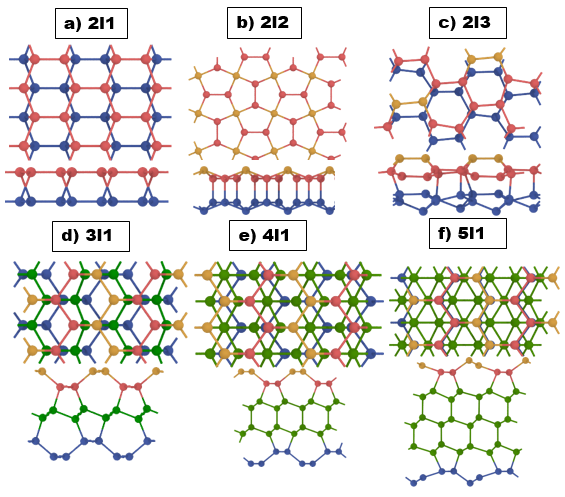
\includegraphics[width=0.48\textwidth]{images/structures}
  \caption{\label{fig:structures}  (color online) Some typical structure of multilayer silicene. Within which  are top view and side view of the studied structures. The buckling atoms on the top surface are labeled as yellow while the red atoms represent the others on the top surface. All the atoms on the bottom surface are labeled as blue. The greens represent those that are inside the structure. The orientation of top view of the cells is labeled as arrows.}
\end{figure}

Before calculating thermal transportation properties , the  structures are  optimized with  conjugate gradient (CG) method which guarantee the stability of them .  Then finite displacement method (FDM) realized in Phonopy\cite{Togo2008} and Thridorder respectively are applied to extract second- and third-order force constants (FCs) in which hundreds of  slightly displaced supercells are generated and their forces are calculated with LAMMPS and used to calculate the FCs with  numerical differential calculation. The chosen supercells is $3 \times 3 \times 1$ of premitive cells to make the inplane dimension above  $40\angstrom$ which make  forces acurrate enough. As for the out-of-plane dimension, according to the previous studies, we choose Si (111) layer spacing of $3.14 \angstrom$ as the thickness of each layer.

The thermal conductivity tensor could be calculated with

\begin{equation}
  \kappa^{\alpha\beta} = \sum_{k \sigma}{c_{k \sigma}v^{\alpha}_{k \sigma}v^{\beta}_{k \sigma}\tau_{k \sigma}} \label{eq:kappasum}
\end{equation}

Where $c_{k \sigma}$ means heat capacity of phonon mode $k \sigma$, $v^{\alpha}$ present for mode group velocity and $\tau_{k \sigma}$ is phonon lifetime. The heat capacity  could be computed with Eq.(\ref{eq:cv}) .

\begin{equation}
  c_{k \sigma}=\frac{\hbar \omega_{k \sigma} }{V} \frac{\partial f(\omega_{k \sigma},T)}{\partial T} \label{eq:cv}
\end{equation}

Where $ f(\omega,T)=1/(exp(\frac{\hbar \omega}{k_b T})-1)$ is Bose-Einstein distribution function.

The calculations of $c_{k\sigma}$ , $v_{k\sigma,\alpha}$, and $\tau_{k\sigma}$ require second- and third-order force constants (FCs) as inputs and the detail formulas are refered to the work of  Wu Li\cite{Li2014}. To avoid underestimate of thermal concutivity,Iteration method is used instead of relaxation time approximision (RTA) .A $45\times 45 \times 1$ Monkhorst-Pack q-point mesh is used to obtain enough phonons for the convergence of the summation as well as for further statistical analysics of them.



\section{RESULTS AND DISCCUSION}

Surface reconstruction is found to have substantial influence on the intensity and anisotropy of thermal conductivity. The relationship between the thermal conductivity  and the length of three kinds of bilayer silicene along different directions is shown in FIG.\ref{fig:tc_length_sheng}(a). The absolute value of the thermal conductivity shows a large gap between these different surface reconstructions. The thermal conductivity of 2l1 structure reaches up to $42.1W/mK$ and $57.9W/mK$ in the zigzag and armchair directions respectively , while those of 2l2 structure are about $31.1W/mK$ in both direction and those of 2lhex structure are around $5W/mK$. 2l2 and 2lhex structures both show large anisotropy while 2l2 does not because 2l2 structure exhibits excellent rotation symmetry of $\frac{\pi}{2}$. The thermal conductivity and anisotropy of multilayer silicene is shown in TABLE.\ref{tab:table1}.   The above results show that surface reconstruction has a significant effect on the thermal transport properties of multilayer silicene. The smooth surface is favorable for heat conduction, while the rough surface can greatly suppress the heat conduction. Meanwhile, the anisotropy of the surface structure leads to the significant anisotropy of the thermal conductivity.


The thermal conductivity converged with cutoff MFP very quickly in the curve of 2l2 while a little slower in the others. Besides, the cutoff MFP of 2l1 structure exhibits much difference in the two directions  which maybe due to the diffence of scattering intensity caused by the surface conditions.When the length of the silicene is smaller than the mean free path of the phonon, the ballistic transport properties of the phonon are obvious. When the length is larger than the mean free path of the phonon, the phonon scattering transport characteristics are obvious. The empirical formula of the John A. Thomas\cite{Thomas2010} can be used to characterize the thermal conductivity of the phonon transport from ballistic to scattering region, at the same time accurately obtaining thermal conductivity of the infinite long nano materials. Using this formula, we obtain the thermal conductivity of infinitely long multilayer silicene
\begin{equation}
  \kappa = \kappa_\infty (1-e^{-\frac{L}{L_c}}) \label{eq:eq_nemd}
\end{equation}

where $\kappa_\infty$ is the fitted full scattering thermal conductivity. $L_c$ is the transition length from the ballistic transportation to the scattering transportation.

\begin{figure}[b]
  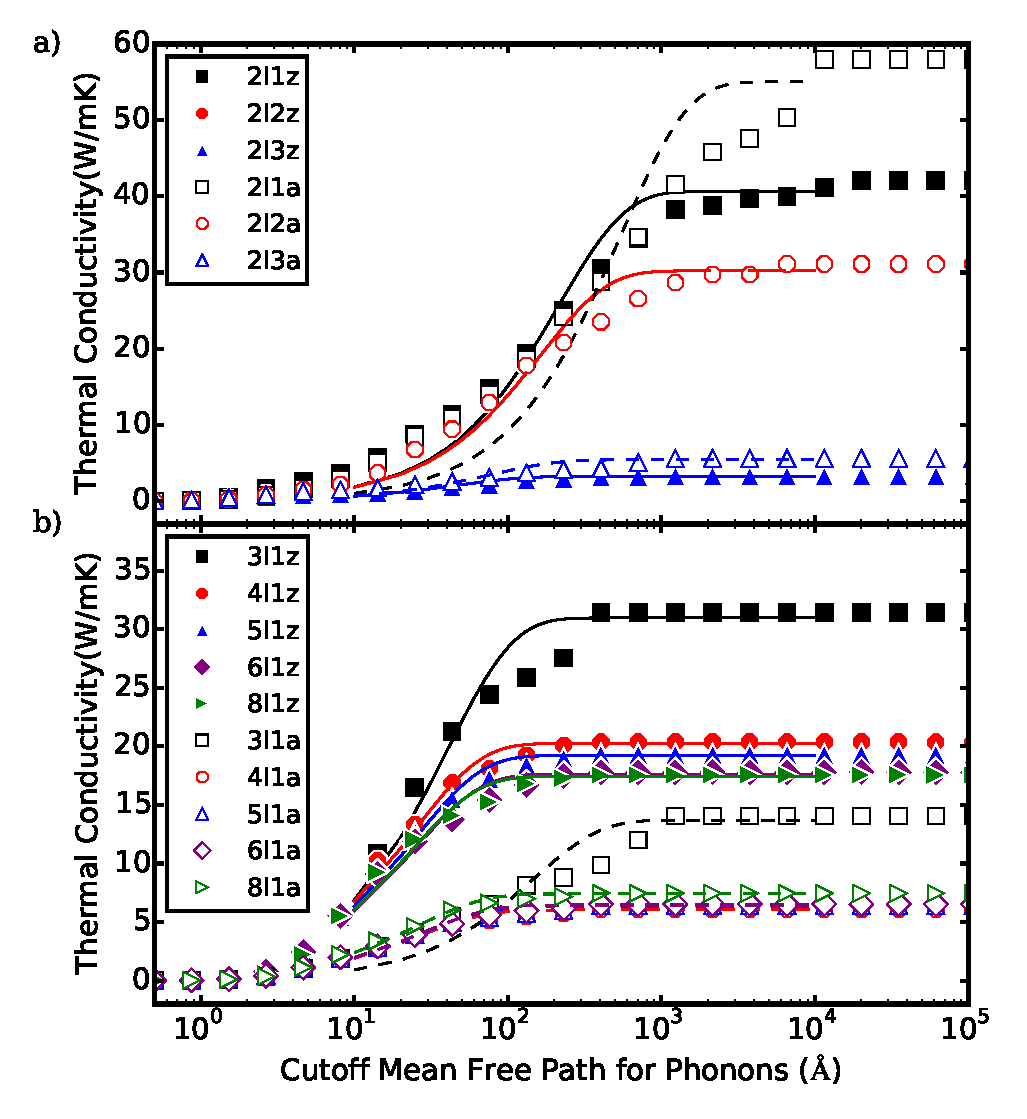
\includegraphics[width=0.48\textwidth]{images/tc_length_sheng}
  \caption{\label{fig:tc_length_sheng} (color online) a) The thermal conductivity dependence on length for three types of bilayer silicene. b) The dependence on length of thermal conductivity for silicene with several layers.The scatters are the results of BTE calculations while the lines are fitted with Eq.(\ref{eq_nemd}). The letter z/a in the legend mean the transport direction is zigzag/armchair.}
\end{figure}




With the increase of layer number the anisotropy decreases for layer number larger than three. Here we study mainly on multilayer silicene structure with 3-8 layers, whose  surface has typical Si (111) $2 \times 1$ surface reconstruction.   From TABLE.\ref{tab:table1}, for the stuctures with more than three layers,the thermal conductivity of the multilayer silicene with zigzag type is higher than that of armchair. $\kappa_z$ decreases while $\kappa_a$ increases. The reason is that the zigzag direction of the multilayer silicene surface is composed of a smooth zigzag atomic chain (as shown in FIG.\ref{fig:structures}). Compared with the bulk silicene structure, the heat conduction along the zigzag direction has no obvious effect on the heat flow. While along the armchair direction, the fluctuation of multilayer silicene surface is very large, the same is its obvious affection on heat flow. This difference is mainly caused by the surface reconstruction effect, and will decrease with the increase of the thickness of the silicene. It's expected that when the layer number reaches infinity the value of them collapse because we finally obtain the bulk phase. The value $ \chi=|\kappa_{z,\infty}-\kappa_{a,\infty} |/max⁡(\kappa_{z,\infty}-\kappa_{a,\infty} ) \times 100 \%$ is used to measure the thermal conductivity difference in different directions, where $ \kappa_{z,\infty} (\kappa_{a,\infty})$ stands for the full scattering thermal conductivity (infinite thermal conductivity) in the zigzag (armchair) direction. And is $ max⁡(\kappa_{z,\infty}-\kappa_{a,\infty} ) $ the maximum value of thermal conductivity in the two directions. The magnitude of the anisotropy $\chi$ is also shown in TABLE.\ref{tab:table1},which  decreases obviously for these structures which is expected. The case of three layers is exceptional whose values are much larger than the structures with those with larger layer number and possesses a smaller anisotropy. This could be understood by the direct interaction beteen the top and bottom sides , and also the absence of hexatomic ring in the side view compared with 4l1 structure.A deeper analysis of this of it could be found in work of Guo \cite{Guo2015Structural}.


On the other hand, the size effect of the thermal conductivity anisotropy is obvious. As shown in FIG.\ref{fig:tc_length_sheng}(b), at the same thickness, in the case of shorter length (10 - 50nm), the anisotropy is obvious. When the length is about 100nm, the anisotropy difference becomes very small. This is essentially due to the difference in the out-of-plane acoustic branch (LA), the transverse acoustic branch (TA), and the vertical plane acoustic phonon (ZA) of the multilayer silicene structures along different directions. However, with the increase of length, the ballistic transport is gradually saturated, and the difference of the heat transfer caused by the umklapp process is gradually reduced.



\begin{table*}
  \caption{\label{tab:table1}
    The thermal conductivity and anisotropic ratio of different multi-layer silicene.Along with the average heat capacity ($kJ/m^3/K$) of zigzag direction and armchair direction.}
  \begin{ruledtabular}
    \begin{tabular}{ccccccc}
          & Minimal period
          & $\kappa_{z,\infty}$
          & $\kappa_{a,\infty}$
          & $\chi$
          & $Cv_{z}$
          & $Cv_{a}$                                                           \\
      \hline
      2l1 & $1 \times 1$             & 42.10 & 57.92 & 27.31\% & 165.8 & 166.7 \\
      2l2 & $\sqrt{2}\times\sqrt{2}$ & 31.11 & 31.11 & 0    \% & 38.44 & 38.44 \\
      2lh & $2 \times 2$             & 3.311 & 5.624 & 41.13\% & 22.42 & 22.42 \\
      3l1 & $2 \times 1$             & 31.44 & 14.05 & 55.29\% & 52.22 & 52.46 \\
      4l1 & $2 \times 1$             & 20.37 & 6.114 & 69.98\% & 37.71 & 37.89 \\
      5l1 & $2 \times 1$             & 19.33 & 6.419 & 66.78\% & 29.17 & 29.32 \\
      6l1 & $2 \times 1$             & 17.78 & 6.527 & 63.29\% & 23.73 & 23.86 \\
      8l1 & $2 \times 1$             & 17.56 & 7.461 & 57.51\% & 17.26 & 17.36 \\
    \end{tabular}
  \end{ruledtabular}
\end{table*}

For the structures of two layers the anisotropy mainly comes from low frequency phonons while that of layer number more than fore are contributed from high frequency phonons. The frequency distribution of thermal conductivity is shown in Fig.\ref{fig:tc_freq} and it's obvious that both 2l1 and 2lhex have much larger value in the low frequency part of armchair direction and they are the only two structures with thermal conductivity of armchair direction larger than that of zigzag direction. For the other structures except 3l1, the low frequency region exhibits little anisotropy while the high frequency thermal condcutivity of zigzag contribution is larger than that of armchair direction. Besides, the curves show much similarity for 4l1,5l1 and 6l1, suggesting a common mechanism of the anisotropy of them.

To have a deeper inside into the origin of anisotropy for all the structures it's helpful to study all the factors that contribute to thermal conductivity according to Eq.(\ref{eq:kappasum}).

Heat capacity has large influence between the structures but has no contribution to anisotropy. We select all the phonons along  $\Gamma\rightarrow X$ and along $\Gamma \rightarrow Y$ and cacluate their heat capacity with Eq.(\ref{eq:cv}). The values are averaged to get $Cv_z$ while those of phonons along $\Gamma\rightarrow Y$ are called $Cv_a$. The average heat capacity of the structures are shown in Table.\ref{tab:table1} . Large difference could be found between the $Cv$ of the structures. The lowest value is $17.26 kJ/m^3/K$ of 8l1 while the highest value of 2l1 could reach $166.7 kJ/m^3/K$, and this could lead to large difference between their thermal conductivity.  Almost no difference could be found in the value along zigzag direction and armchair direction. This is due to the insensitivity of heat capacity to frequency when the frequency is low and the value is ignorable when frequency is relatively high, which means when considering only acoustic phonons the heat capacity is close to constant.

\begin{figure}[b]
  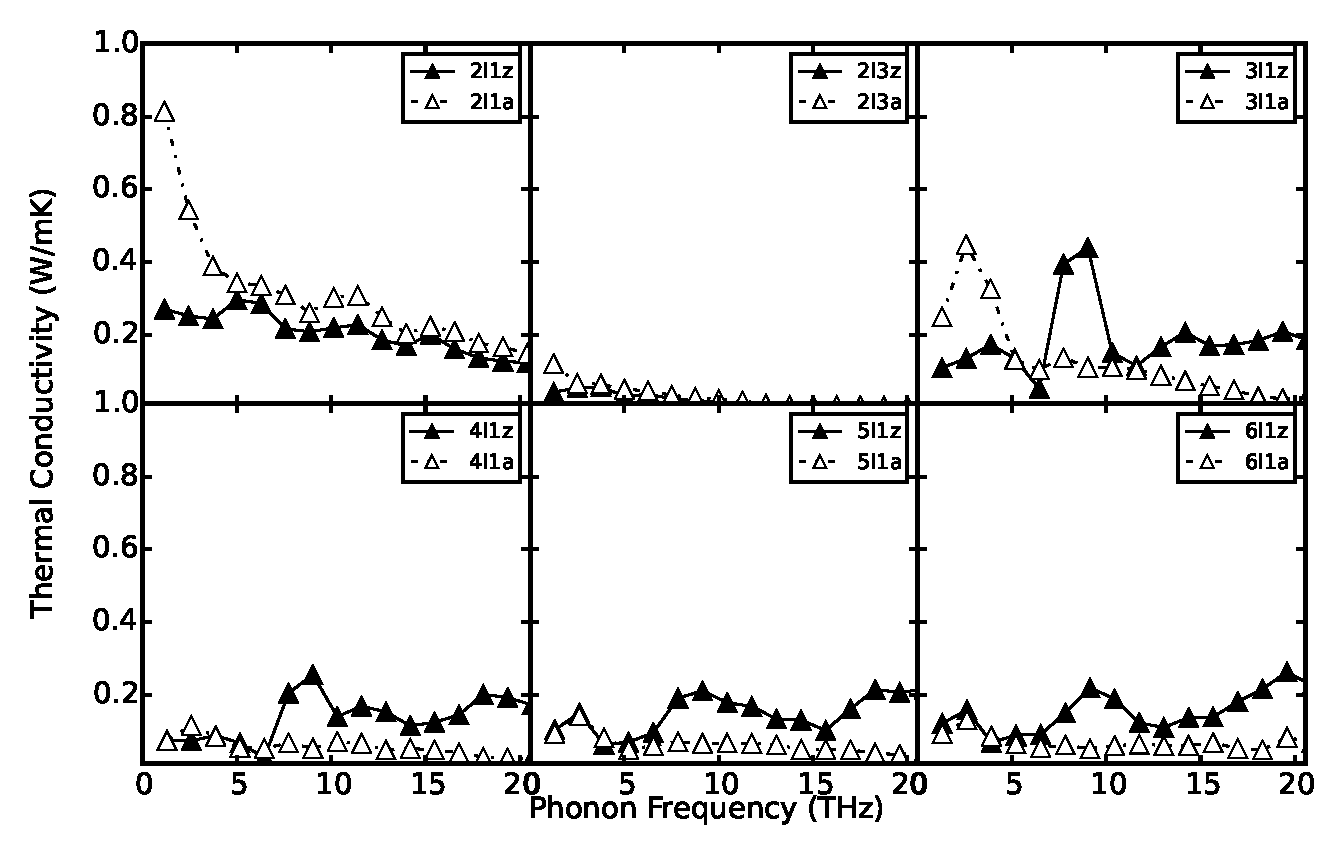
\includegraphics[width=0.48\textwidth]{images/tc_freq}
  \caption{\label{fig:tc_freq} (color online)  The converged thermal conductivity versus phonon frequency of the structures. }
\end{figure}

\begin{figure}[b]
  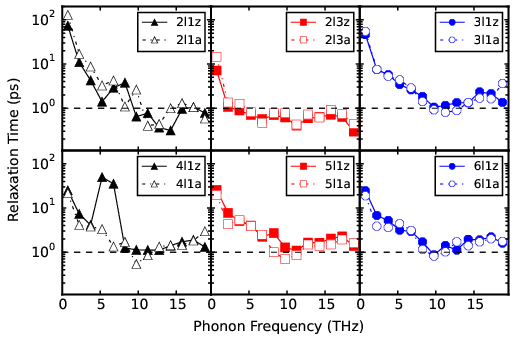
\includegraphics[width=0.48\textwidth]{images/tau}
  \caption{\label{fig:tau} (color online)Lifetime of phonons considering three-phonon scattering for all the structures. }
\end{figure}


The phonon lifetimes are the main factor of anisotropy in two layer structures while they are less essential in that of structures with more than three layers. When calutating phonon lifetimes, only three-phonon scattering process are considered,which consists of two types of scattering processes, within one of which  two phonons vanish and one phonon be created and the other type is one phonon transform to two phonons. Both of them are possible to have result phonons with q point outside Brillouin boundry, which must be fold back to Brillouin zone to make the result physcical( $\mathbf{q''}=\mathbf{q} \pm \mathbf{q'}+\mathbf{G}$). So this process is called Umpack process( U process). And of cause there exist  situation that none of the three q points outside the Brillouin boundry, and the summation of the momentum conserves ( $\mathbf{q''}=\mathbf{q} \pm \mathbf{q'}$), which is called Normal process (N process) or momentum conservation process. If there's no U process the thermal conductivity could be as large as possible, so this process gives the dominent contribution to thermal resistance. The phonon scattering rate could be obtained by Fermi-golden rule\cite{Li2014} considering only the relaxation time approxmition(RTA). We then use iterative method to consider in cross influence of the phonon exitatioin, witch always give lager lifetime compare to RTA and more close to the real value. The phonon lifetime calculated with ShengBTE\cite{Li2014} are shown in FIG.\ref{fig:tau}. The values are averaged for frequency bins to reduce complexity. The lifetime of 3l1,4l1,5l1,6l1 along zigzag direction is larger than armchair direction while that of 2l1,2lh has reverse relation. However the anitropy of lifetime  is quite obvious in two layers structures , where lifetime of armchair direction is larger almost through all the frequency, while there's not much anisotropy in multilayer structures expcet in the 4THz-7THz range of 4l1 structure.

\begin{figure}[b]
  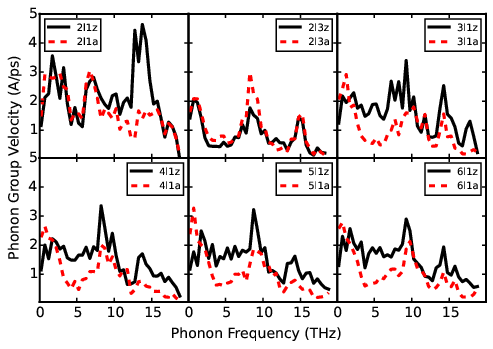
\includegraphics[width=0.48\textwidth]{images/gv}{}
  \caption{\label{fig:gv} (color online)Group Velocity versus phonon frequencies for both zigzag direction and armchair direction of the structures.The histogram bin width is chosen as 1.5THz.}
\end{figure}

While the anisotropy lifetime in two layer structures affects more than that of group velocity, group velocity contributes most of anisotropy in multilayer structures with layers more than three.  FIG.\ref{fig:gv} showes the group velocity along both zigzag and armchair direction for all the structures. The group velocity  along the two directions of  2 layers silicene ( include silicene) are basicly the same except for the frequency range of 12THz - 15THz in 2l1 structure whose  group velocities are highly anisotropic. Group velocity for the others exhibits similar curve and are all highly anisotropic both in low and high frequency range. The group velocity of zigzag direction are all large than that of zigzag. These results  show that the main effect of anistropy is not from group velocity but the scatter rate origin from anharmonic effects in two layer silicene but the reverse for the structures thicker.

\begin{figure}[b]
  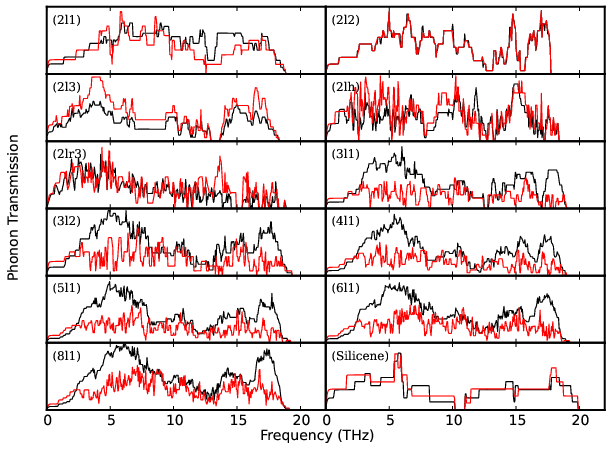
\includegraphics[width=0.48\textwidth]{images/transmission}
  \caption{\label{fig:transmission} (color online)The anisotropic transmission function of the structures. The structure identifiers are labeled at top-left of each subplot. the transmission along zigzag direction is ploted as black curve while that of armchair direction is filled. The y range of each subplot is normalized to the max value within the graph.}
\end{figure}

Not only group velocity,but also phonon transmission clearly show that  localization of ballistic contribution from long wave phonons dominant the anisotropy of the structures with layers more than three.To quatitily study the number of transmission channels we use Non-Equalibrium Green Function (NEGF)\cite{Mingo2003} to calculate the transmission function of the struction along zigzag and armchair direction.The transmission function can be expressed as
\begin{equation}
  \begin{split}
    \Theta(\omega)= Tr(
    \mathbf{\widetilde{k}}_{a\alpha}
    Im(\mathbf{g}_{\alpha\alpha})
    \mathbf{\widetilde{k}}_{\alpha a}
    \mathbf{G}_{a b}^*\\
    \mathbf{\widetilde{k}}_{b\beta}
    Im(\mathbf{g}_{\beta\beta})
    \mathbf{\widetilde{k}}_{\beta b}
    \mathbf{G}_{b a}
    )
  \end{split}
\end{equation}
where $\mathbf{\widetilde{k}}_{a\alpha}$,$\mathbf{\widetilde{k}}_{\alpha a}$ represents for the interaction between left lead and center region and its transposition,  $\mathbf{\widetilde{k}}_{b\beta}$,$\mathbf{\widetilde{k}}_{\beta b}$ the interaction between center and right lead. $\mathbf{g}$ and $\mathbf{G}$ the retarded Green's function of the leads and center rigion.$Tr$ and $Im$ means trace and imaginary function. Transmission function represents for the number of channels of a given frenquency. The more chanels means larger capability of thermal transportation. The value is substracted by the cross area of the transportation direction to eliminate the effect of lattice constants.FIG.\ref{fig:transmission} shows the phonon transmission function along both zigzag and armchair directions. The y-axis value of each panel is scaled for a more convinient comparison of transmission in the tow directions. The steps in the curves are  characterisic of perfection of the structure. Defects like isotope or grain boundary could lead to disapearance of these step.The transmission of  2l1 is perfectly stepwise because of the perfect bonding and the absence of disorder.Transmission of both directions of 2l1 ,2l2(not show here) and 2lh are close,especially that of 2l2 are exactly the same due to the structure symmetry of it.The anistropy of the transmission are clearly found in other structure such as 3l1,4l1,5l1 and 6l1 where transmissioin is larger in zigzag direction than in armchair. This trends is quite consist with that of the thermal conducivity so transmission indeed has large effection on the difference of thermal conductivity. The transmission along zigzag direction has a large peak at around 5THz in the structure 3l1,3l2,4l1,5l1,6l1,8l1,while along armchair direction the peak vanish and this contributes a lot to the anisotropy of the thermal transportation.


To obtain a clear connection between  the surface characteristic we also statistic the force constants of different position of the structures.



\section{CONCLUSIONS}

By means of Boltzmann Transporation Equation (BTE) methods, we found that the thermal transport properties of multilayer silicene structures have significant surface effect and size effect in thickness direction. Under the influence of double layer surface reconstruction, the thermal conductivity of the bilayer silicene can reach up to 57.92 W/mK (2l1 structure), and can be as low as 3.31 W/mK (2lh structure) and the anisotropy can be as high as 41.1\%. The smooth surface is favorable for heat conduction, while the rough surface can greatly suppress the heat conduction. The ultra-low thermal conductivity indicates that the bilayer silicene 2lh has good thermoelectric properties. In the 3-8 layer multilayer silicene with the same $2 \times 1$ surface reconstruction the zigzag direction is more heat conducive. With the increase of the number of layers, the thermal conductivity of the zigzag direction decrease, but the thermal conductivity increased a little in the armchair direction, and the anisotropy of thermal conductivity decreased. The anisotropy mainly comes from phonon scattering effect in bilayer structures while the anisotropy mainly comes from localization of ballistic phonons in 3-8 layer multilayer silicene which could be charactered by phonon group velocity and NEGF transmission function. This work could be helpful in the field of heat management, thermoelectric applications involving silicene and other multilayer nano materials in the future.

\quad \\
\section{ACKNOWLEGEMENTS}
This paper was partially supported by the National Natural Science Foundation of China, the Special Funds for Major State Basic Research, the Foundation for the Author of National Excellent Doctoral Dissertation of China, the Program for Professor of Special Appointment at Shanghai Institutions of Higher Learning, and the Research Program of Shanghai Municipality and the Ministry of Education.


\bibliography{ref}
\end{document}
